%------------------------------------------
%	$Id: GMT_Chapter_7.tex,v 1.64 2010-01-05 03:49:47 guru Exp $
%
%	The GMT Documentation Project
%	Copyright 2000-2010.
%	Paul Wessel and Walter H. F. Smith
%------------------------------------------
%
\chapter{Creating GMT Graphics}
\label{ch:7}
\thispagestyle{headings}

In this section we will be giving several examples of
typical usage of \GMT\ programs.  In general, we will
start with a raw data set, manipulate the numbers in
various ways, then display the results in diagram or
map view.  The resulting plots will have in common that
they are all made up of simpler plots that have been
overlaid to create a complex illustration.  We will
mostly follow the following format:

\begin{enumerate}
\item We explain what we want to achieve in plain
language.

\item We present an annotated Bourne shell script that contains
all commands used to generate the illustration.

\item We explain the rationale behind the commands.

\item We present the illustration, 50\% reduced in size, and without
the timestamp (\Opt{U}).
\end{enumerate}

A detailed discussion of each command is not given;
we refer you to the manual pages for command line
syntax, etc.  We encourage you to run these scripts for yourself.
See Appendix~\ref{app:D} if you would like an electronic version
of all the shell-scripts (both \progname{sh} and \progname{csh} scripts
are available, as or DOS batch files; only the \progname{sh}-scripts are discussed here) and support
data used below.  Note that all examples explicitly specifies the
measurement units, so although we use inches you should be able
to run these scripts and get the same plots even if you have cm
as the default measure unit.  The examples are all written to be ``quiet'',
that is no information is echoed to the screen.  Thus,
these scripts are well suited for background execution.

Note that we also end each script by cleaning up after
ourselves. Because \progname{awk} is broken as designed on some
systems, and \progname{nawk} is not available on others we refer
to \progname{\$AWK} in the scripts below; the \progname{do\_examples.sh}
scripts will set this when running all examples. 

Finally, be aware that for practical purposes the output \PS\ file name is stored as the variable \texttt{ps}.

\section{The making of contour maps}

\index{Example!contour maps|(}

We want to create two contour maps of the low order geoid
using the Hammer equal area projection.  Our gridded data
file is called \filename{osu91a1f\_16.grd} and contains a global 1\DS\ 
by 1\DS\ gridded geoid (we will see how to make gridded
files later).  We would like to show one map centered on
Greenwich and one centered on the dateline.  Positive contours
should be drawn with a solid pen and negative contours with
a dashed pen.  Annotations should occur for every 50 m contour
level, and both contour maps should show the continents in
light gray in the background.  Finally, we want a rectangular
frame surrounding the two maps.  This is how it is done:

\script{example_01} 

The first command draws a box surrounding the maps.  This is
followed by two sequences of
\GMTprog{pscoast}, \GMTprogi{grdcontour}, \GMTprogi{grdcontour}.
They differ in that the first is centered on Greenwich; the
second on the dateline.  We use the limit option (\Opt{L})
in \GMTprog{grdcontour} to select negative contours only and plot
those with a dashed pen, then positive contours only and draw
with a solid pen [Default].  The \Opt{T} option causes tickmarks
pointing in the downhill direction to be drawn on the innermost,
closed contours.  For the upper panel we also added - and + to
the local lows and highs.  You can find this illustration as
Figure~\ref{fig:GMT_example_01}.

\GMTexample{01}{Contour maps of gridded data.}

\index{Example!contour maps|)}

\section{Image presentations}
\label{sec:example_02}
\index{Example!image presentations|(}

As our second example we will demonstrate how to make color
images from gridded data sets (again, we will defer the
actual making of grid files to later examples).  We will
use the supplemental program \GMTprog{grdraster} to extract 2-D
grid files of bathymetry and Geosat geoid heights and put the
two images on the same page.  The region of interest is the
Hawaiian islands, and due to the oblique trend of the island
chain we prefer to rotate our geographical data sets using
an oblique Mercator projection defined by the hotspot pole
at (68\DS W, 69\DS N).  We choose the point (190\DS ,
25.5\DS ) to be the center of our projection (e.g., the
local origin), and we want to image a rectangular region
defined by the longitudes and latitudes of the lower left
and upper right corner of region.  In our case we choose
(160\DS , 20\DS ) and (220\DS , 30\DS ) as the
corners.  We use \GMTprog{grdimage} to make the illustration:

\script{example_02} 

The first step extracts the 2-D data sets from the local
data base using \GMTprog{grdraster}, which is a supplemental
utility program (see Appendix~\ref{app:A}) that may be adapted to
reflect the nature of your data base format.  It
automatically figures out the required extent of the region
given the two corners points and the projection.  The extreme
meridians and parallels enclosing the oblique region is
\Opt{R}159:50/220:10/3:10/47:35.  This is
the area extracted by \GMTprog{grdraster}.  For your convenience
we have commented out those lines and provided the two
extracted files so you do not need \GMTprog{grdraster} to try
this example.  By using the embedded grid file format
mechanism we saved the topography using kilometers as the
data unit.  We now have two grid files with bathymetry and
geoid heights, respectively.  We use \GMTprog{makecpt} to generate
a linear color palette file \filename{geoid.cpt} for the geoid and use
\GMTprog{grd2cpt} to get a histogram-equalized cpt file \filename{topo.cpt}
for the topography data.  To emphasize the structures in
the data we calculate the slopes in the north-south direction
using \GMTprog{grdgradient}; these will be used to modulate the
color image.  Next we run \GMTprog{grdimage} to create a
color-code image of the Geosat geoid heights, and draw a
color legend to the right of the image with \GMTprog{psscale}.
Similarly, we run \GMTprog{grdimage} but specify \Opt{Y}4.5i
to plot above the previous image.  Adding scale and label
the two plots a) and b) completes the illustration
(Figure~\ref{fig:GMT_example_02}).
\index{Example!image presentations|)}
\GMTexample{02}{Color images from gridded data.}

\section{Spectral estimation and xy-plots}
\index{Example!spectral estimation|(}
\index{Example!xy plots|(}

In this example we will show how to use the \GMT\ programs
\GMTprog{fitcircle}, \GMTprog{project}, \GMTprog{sample1d},
\GMTprog{spectrum1d}, \GMTprog{psxy}, and \GMTprog{pstext}.
Suppose you have (lon, lat, gravity) along a satellite track
in a file called \filename{sat.xyg}, and (lon, lat, gravity)
along a ship track in a file called \filename{ship.xyg}.
You want to make a cross-spectral analysis of these data.
First, you will have to get the two data sets into equidistantly
sampled time-series form.  To do this, it will be convenient to
project these along the great circle that best fits the sat track.
We must use \GMTprog{fitcircle} to find this great circle and choose
the L$_2$  estimates of best pole.  We project the data using
\GMTprog{project} to find out what their ranges are in the projected
coordinate.  The \GMTprog{minmax} utility will report the minimum and
maximum values for multi-column ASCII tables.  Use this information
to select the range of the projected distance coordinate they have
in common.  The script prompts you for that information after
reporting the values.  We decide to make a file of equidistant
sampling points spaced 1 km apart from -1167 to +1169, and use
the \UNIX\ utility \progname{\$AWK} to accomplish this step.  We can then
resample the projected data, and carry out the cross-spectral
calculations, assuming that the ship is the input and the satellite
is the output data.  There are several intermediate steps that
produce helpful plots showing the effect of the various processing
steps (\filename{example\_03[a--f].ps}), while the final plot
\filename{example\_03.ps} shows
the ship and sat power in one diagram and the coherency on another
diagram, both on the same page.  Note the extended use of
\GMTprog{pstext} and \GMTprog{psxy} to put labels and legends directly on
the plots.  For that purpose we often use \Opt{Jx}1i and specify
positions in inches directly.  Thus, the complete automated
script reads:

\script{example_03} 

The final illustration (Figure~\ref{fig:GMT_example_03}) shows that the ship gravity
anomalies have more power than altimetry derived gravity for
short wavelengths and that the coherency between the two
signals improves dramatically for wavelengths $>$ 20 km.
\GMTexample{03}{Spectral estimation and $x/y$-plots.}

\index{Example!spectral estimation|)}
\index{Example!xy plots|)}

\section{A 3-D perspective mesh plot}
\index{Example!3-D mesh plot|(}

This example will illustrate how to make a fairly complicated
composite figure.  We need a subset of the ETOPO5 bathymetry\footnote{
These data are available on CD-ROM from NGDC (www.ngdc.noaa.gov).}
and Geosat geoid data sets which we will extract from the local
data bases using \GMTprog{grdraster}.  We would like to show a
2-layer perspective plot where layer one shows a contour map
of the marine geoid with the location of the Hawaiian islands
superposed, and a second layer showing the 3-D mesh plot of
the topography.  We also add an arrow pointing north and some
text.  This is how to do it:

\script{example_04} 

The purpose of the color palette file \filename{zero.cpt} is to have
the positive topography mesh painted light gray (the remainder
is white). The left side of Figure~\ref{fig:GMT_example_04} shows the complete illustration.

\begin{figure}[ht]
   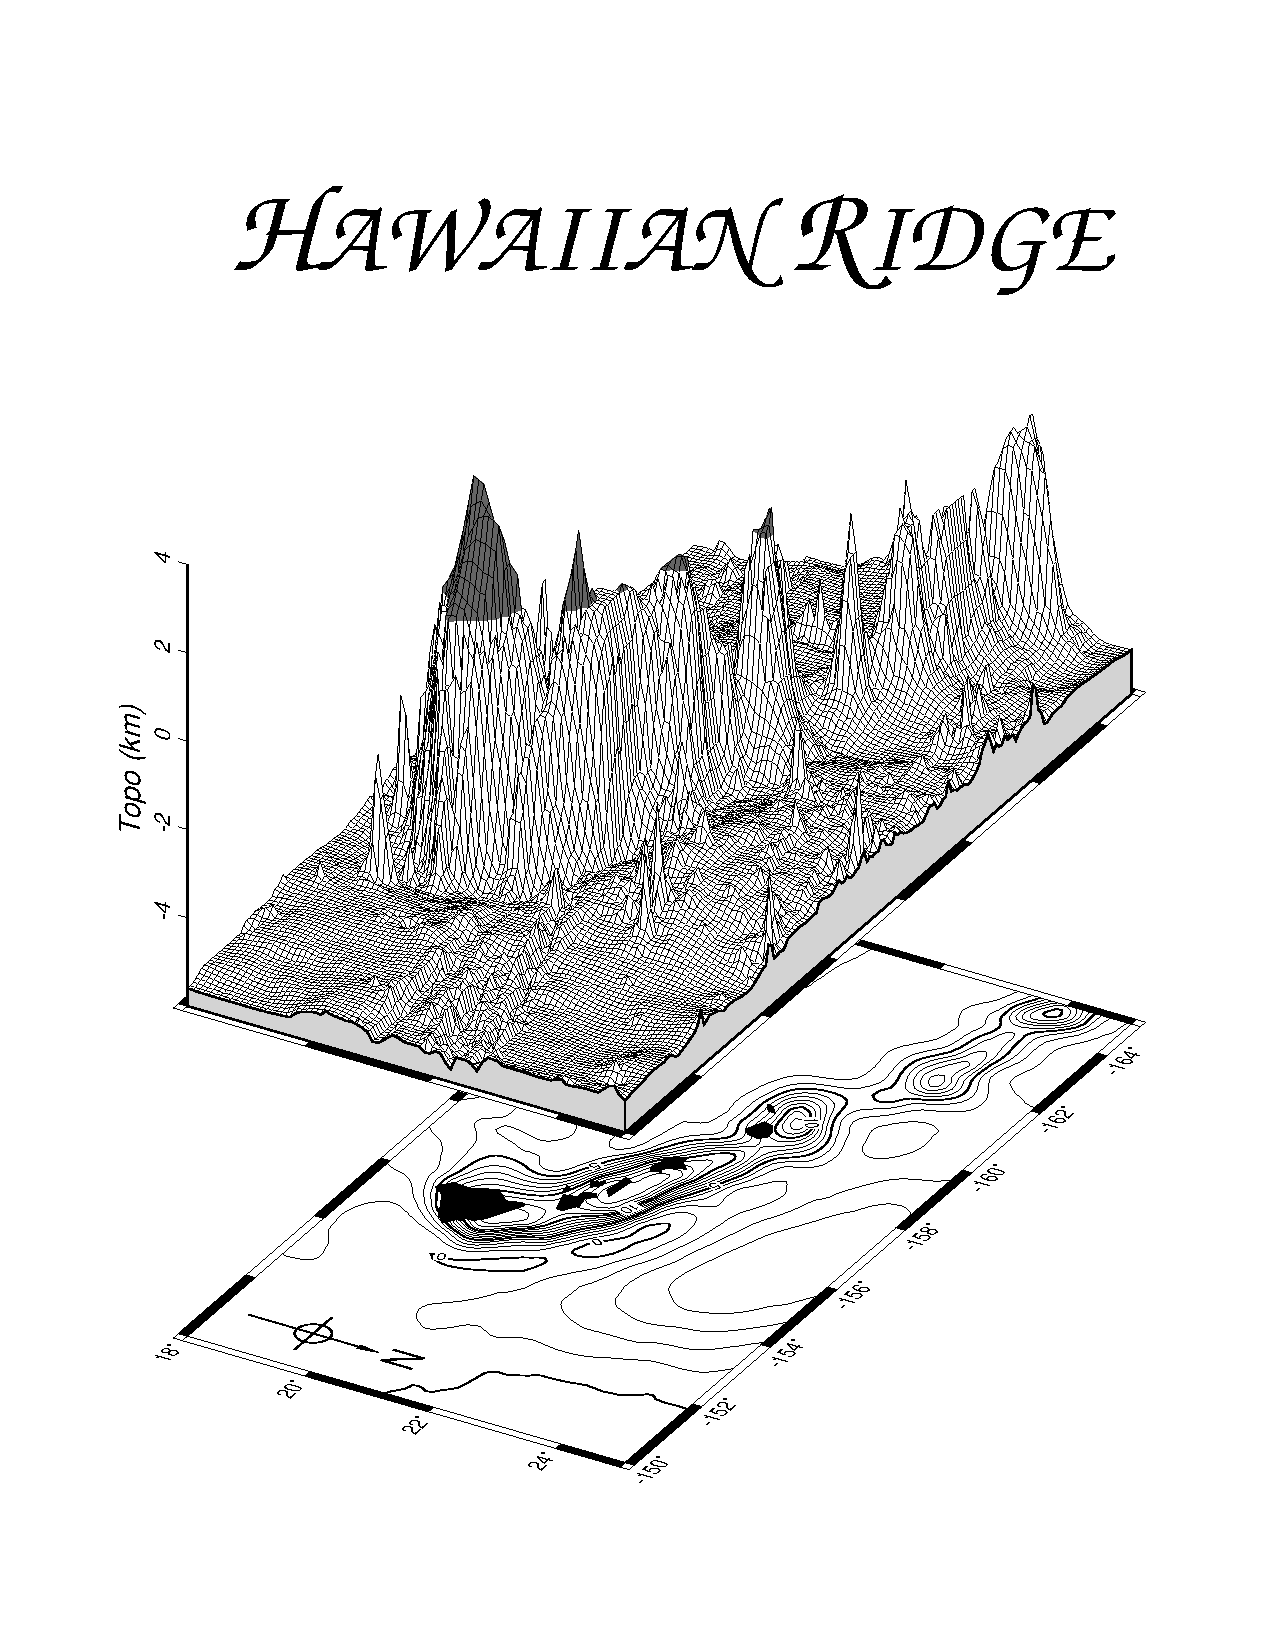
\includegraphics[scale=0.42]{scripts/example_04}\hfill
   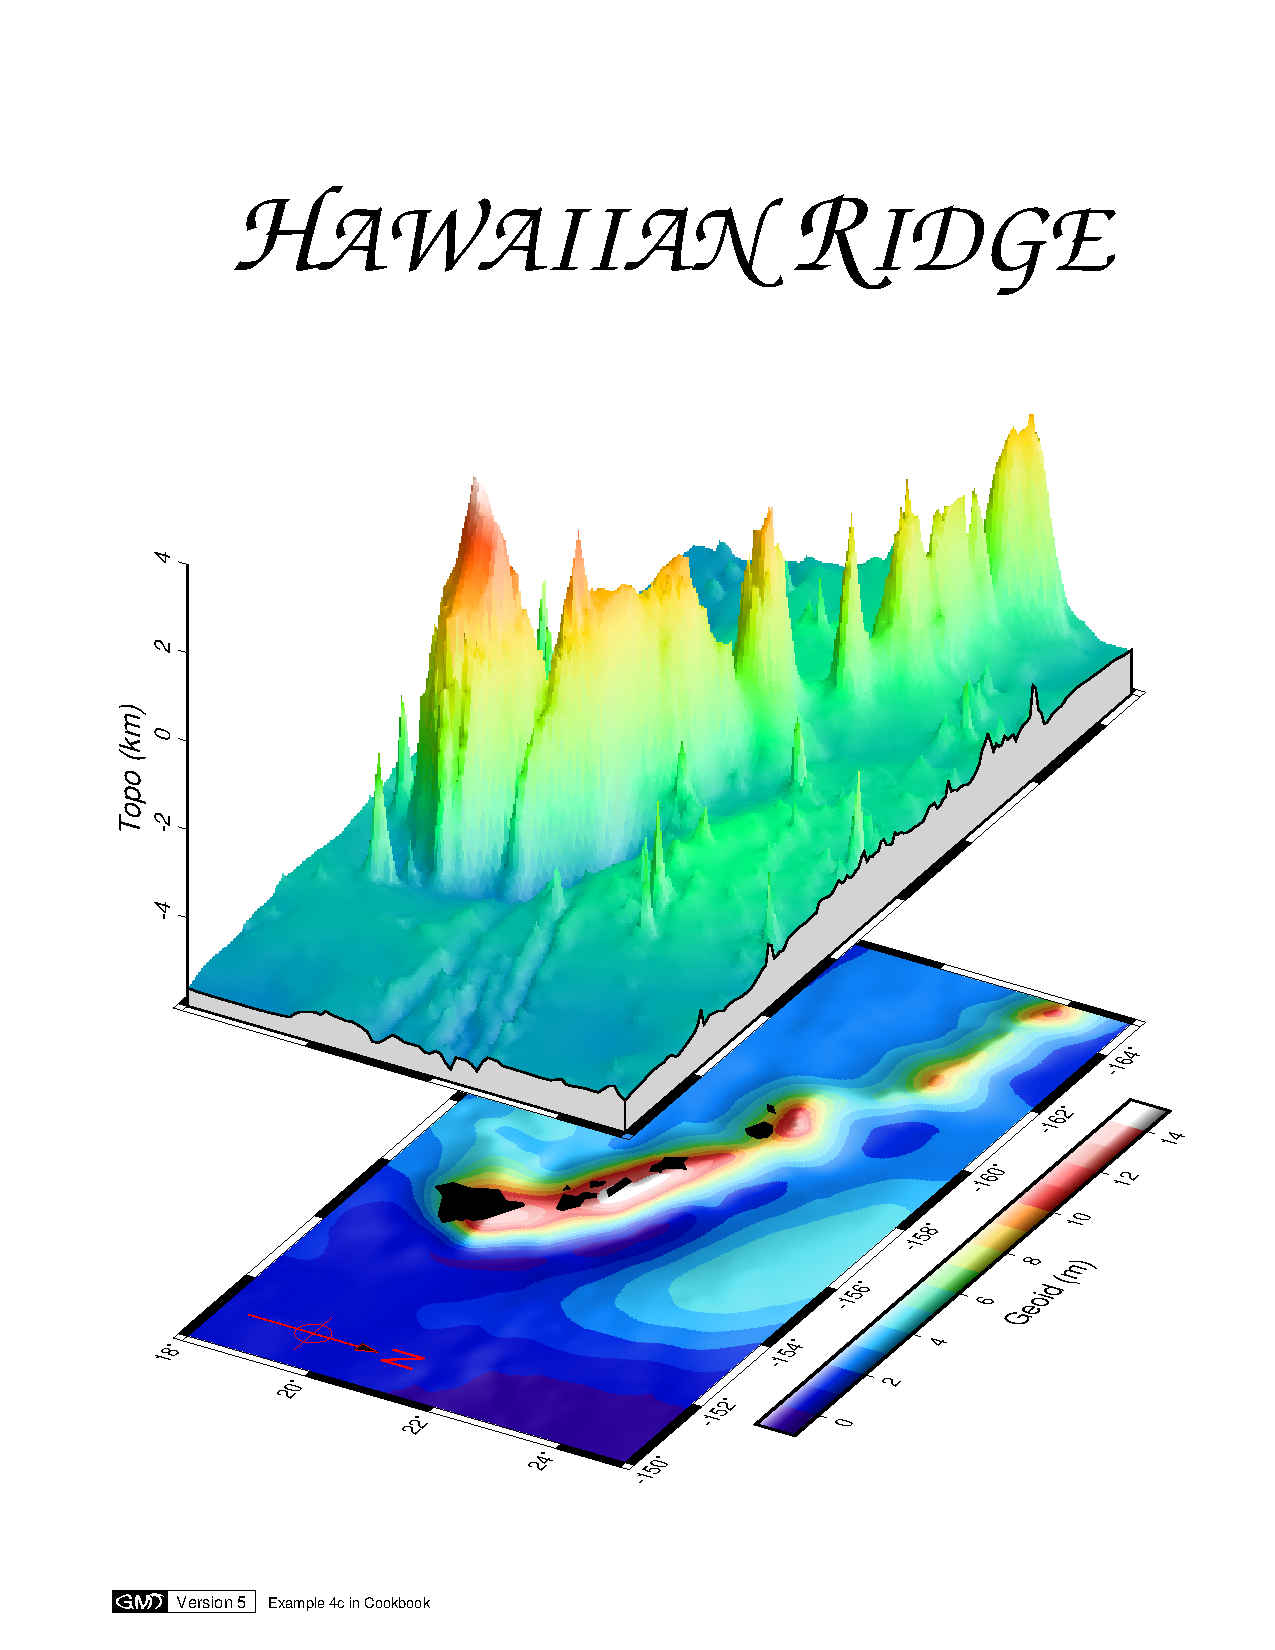
\includegraphics[scale=0.42]{scripts/example_04c}
   \caption{3-D perspective mesh plot (left) and colored version (right).}
   \label{fig:GMT_example_04}
\end{figure}

A color version of this figure was used in our first article in \emph{EOS
Trans. AGU} (Oct. 8th, 1991).  It was created along similar
lines, but instead of a mesh plot we chose a color-coded surface
with artificial illumination from a light-source due north.
We choose to use the \Opt{Qi} option in \GMTprog{grdview} to
achieve a high degree of smoothness.  Here, we select 100 dpi
since that will be the resolution of our final raster
(The EOS raster was 300 dpi). We used \GMTprog{grdgradient} to
provide the intensity files.  The following script creates
the color \PS\ file.  Note that the size of the
resulting output file is directly dependent on the square of
the dpi chosen for the scanline conversion.  A higher value
for dpi in \Opt{Qi} would have resulted in a much larger
output file.  The cpt files were taken from Section~\ref{sec:example_02}.

\script{example_04c} 

\index{Example!3-D mesh plot|)}

\section{A 3-D illuminated surface in black and white}
\index{Example!3-D illuminated surface|(}

Instead of a mesh plot we may choose to show 3-D surfaces using
artificial illumination.  For this example we will use
\GMTprog{grdmath} to make a grid file that contains the surface given
by the function $z(x, y) = \cos (2\pi r/8)\cdot e^{-r/10}$, where
$r^2 = (x^2 + y^2)$.  The illumination is obtained by passing
two grid files to \GMTprog{grdview}: One with the {\it z}-values
(the surface) and another with intensity values (which should
be in the \PM 1 range).  We use \GMTprog{grdgradient} to compute
the horizontal gradients in the direction of the artificial
light source.  The \filename{gray.cpt} file only has one line that states
that all {\it z} values should have the gray level 128.  Thus,
variations in shade are entirely due to variations in gradients,
or illuminations.  We choose to illuminate from the SW and view
the surface from SE:

\script{example_05} 

The variations in intensity could be made more dramatic by
using \GMTprog{grdmath} to scale the intensity file before
running \GMTprog{grdview}.  For very rough data sets one may
improve the smoothness of the intensities by passing the
output of \GMTprog{grdgradient} to \GMTprog{grdhisteq}.  The
shell-script above will result in a plot like the one in
Figure~\ref{fig:GMT_example_05}.

\GMTexample{05}{3-D illuminated surface.}

\index{Example!3-D illuminated surface|)}

\section{Plotting of histograms}
\index{Example!histograms|(}

\GMT\ provides two tools to render histograms: \GMTprog{pshistogram}
and \GMTprog{psrose}.  The former takes care of regular histograms
whereas the latter deals with polar histograms (rose diagrams,
sector diagrams, and wind rose diagrams).  We will show an
example that involves both programs.  The file \filename{fractures.yx}
contains a compilation of fracture lengths and directions as
digitized from geological maps.  The file \filename{v3206.t} contains
all the bathymetry measurements from {\it Vema} cruise 3206.
Our complete figure (Figure~\ref{fig:GMT_example_06}) was made running
this script:

\script{example_06} 
\GMTexample{06}{Two kinds of histograms.}

\index{Example!histograms|)}

\section{A simple location map}
\index{Example!location map|(}

Many scientific papers start out by showing a location map
of the region of interest. This map will typically also
contain certain features and labels.  This example will
present a location map for the equatorial Atlantic ocean,
where fracture zones and mid-ocean ridge segments have been
plotted.  We also would like to plot earthquake locations
and available isochrons.  We have obtained one file,
\filename{quakes.xym}, which contains the position and magnitude of
available earthquakes in the region.  We choose to use
magnitude/100 for the symbol-size in inches.  The digital
fracture zone traces (\filename{fz.xy}) and isochrons (0 isochron as
\filename{ridge.xy}, the rest as \filename{isochrons.xy}) were digitized from
available maps\footnote{These data are available on CD-ROM from NGDC (www.ngdc.noaa.gov).}.
We create the final location map
(Figure~\ref{fig:GMT_example_07}) with the following script:

\script{example_07} 
\GMTexample{07}{A typical location map.}

The same figure could equally well be made in color, which
could be rasterized and made into a slide for a meeting
presentation.  The script is similar to the one outlined
above, except we would choose a color for land and oceans,
and select colored symbols and pens rather than black and white.

\index{Example!location map|)}

\section{A 3-D histogram}
\index{Example!3-D histogram|(}

The program \GMTprog{psxyz} allows us to plot three-dimensional
symbols, including columnar plots.  As a simple demonstration,
we will convert a gridded netCDF of bathymetry into an
ASCII $xyz$ table and use the height information to draw a
2-D histogram in a 3-D perspective view.  Our gridded
bathymetry file is called \filename{topo.grd} and covers the region
from 0 to 5 \DS E and 0 to 5 \DS N.  Depth ranges from
-5000 meter to sea-level.  We produce the Figure~\ref{fig:GMT_example_08} by
running this script:

\script{example_08} 
\GMTexample{08}{A 3-D histogram.}

\index{Example!3-D histogram|)}

\section{Plotting time-series along tracks}
\index{Example!wiggles|(}

A common application in many scientific disciplines involves
plotting one or several time-series as as ``wiggles'' along
tracks.  Marine geophysicists often display magnetic anomalies
in this manner, and seismologists use the technique when
plotting individual seismic traces.  In our example we will
show how a set of Geosat sea surface slope profiles from the
south Pacific can be plotted as ``wiggles'' using the
\GMTprog{pswiggle} program. We will embellish the plot with track
numbers, the location of the Pacific-Antarctic Ridge, recognized
fracture zones in the area, and a ``wiggle'' scale.  The
Geosat tracks are stored in the files \filename{*.xys}, the ridge in
\filename{ridge.xy}, and all the fracture zones are stored in the multiple
segment file \filename{fz.xy}.  We extract the profile id (which is the
first part of the file name for each profile) and the last point
in each of the track files to construct an input file for
\GMTprog{pstext} that will label each profile with the track
number.  We know the profiles trend approximately N40\DS E
so we want the labels to have that same orientation (i.e., the
angle with the baseline must be 50\DS ).  We do this by
extracting the last record from each track, paste this file
with the \filename{tracks.lis} file, and use \progname{\$AWK} to create the
format needed for \GMTprog{pstext}.  Note we offset the positions
by -0.05 inch with \Opt{D} in order to have a small gap
between the profile and the label:

\script{example_09} 

The output shows the sea-surface slopes along 42 descending
Geosat tracks in the Eltanin and Udintsev fracture zone
region in a Mercator projection (Figure~\ref{fig:GMT_example_09}).
\GMTexample{09}{Time-series as ``wiggles'' along a track.}

\index{Example!wiggles|)}

\section{A geographical bar graph plot}
\index{Example!bar graph|(}

Our next and perhaps most business-like example presents a
three-dimensional bar graph plot showing the geographic
distribution of the membership in the American Geophysical
Union (AGU).  The input data was taken from the January 2008 AGU
member directory and added up to give total members per
continent.  We decide to plot a 3-D column centered on
each continent with a height that is proportional to the
logarithm of the membership.  A log$_{10}$-scale is
used since the memberships vary by almost 3 orders of
magnitude.  We choose a plain linear projection for the
basemap and add the columns and text on top. Our script that produces Figure~\ref{fig:GMT_example_10} reads:

\script{example_10}
\GMTexample{10}{Geographical bar graph.}

\index{Example!bar graph|)}

\section{Making a 3-D RGB color cube}
\index{Example!3-D RGB color cube|(}

In this example we generate a series of 6 color images,
arranged so that they can be cut out
and assembled into a 3-D color cube.  The six faces of
the cube represent the outside of the R-G-B color space.
On each face one of the color components is fixed at either
0 or 255 and the other two components vary smoothly across
the face from 0 to 255.  The cube is configured as a
right-handed coordinate system with \emph{x-y-z} mapping
R-G-B.  Hence, the 8 corners of the cube represent the
primaries red, green, and blue, plus the secondaries cyan,
magenta and yellow, plus black and white.

The 6 color faces are generated by feeding \GMTprog{grdimage} three grids, one for each color
component (R, G, and B). In some cases the X or Y axes of a face are reversed by specifying a
negative width or height in order to change the variation of the color value in that direction from
ascending to descending, or vice versa.

A number of rays emanating from the white and black corners indicate the Hue value (ranging from 0 to
360\DS). The dashed and dotted lines near the white corner reflect saturation levels, running from 0
to 1 (in black font). On these 3 faces the brightness is a constant value of 1.
On the other 3 faces of the cube, around the black corner, the white decimal numbers indicate
brightnesses between 0 and 1, with saturation fixed at 1.

Here is the shell script to generate the RGB cube in Figure~\ref{fig:GMT_example_11}:

\script{example_11} 
\GMTexample[width=\textwidth]{11}{The RGB color cube.}

\index{Example!3-D RGB color cube|)}

\section{Optimal triangulation of data}
\label{sec:example_12}
\index{Example!triangulation|(}

Our next example (Figure~\ref{fig:GMT_example_12})
operates on a data set of topographic
readings non-uniformly distributed in the plane (Table
5.11 in Davis: {\it Statistics and Data Analysis in Geology},
J. Wiley).  We use \GMTprog{triangulate} to perform the optimal
Delaunay triangulation, then use the output to draw the
resulting network.  We label the node numbers as well as
the node values, and call \GMTprog{pscontour} to make a contour
map and image directly from the raw data.  Thus, in this
example we do not actually make grid files but still
are able to contour and image the data.  We use a color
palette table \filename{topo.cpt} (created via \GMTprog{minmax} and \GMTprog{makecpt}).
The script becomes:

\script{example_12} 
\GMTexample{12}{Optimal triangulation of data.}

\index{Example!triangulation|)}

\section{Plotting of vector fields}
\index{Example!vector fields|(}

In many areas, such as fluid dynamics and elasticity,
it is desirable to plot vector fields of various kinds.
\GMT\ provides a way to illustrate 2-component vector fields
using the \GMTprog{grdvector} utility.  The two components of
the field (Cartesian or polar components) are stored in
separate grid files.  In this example we use \GMTprog{grdmath}
to generate a surface $z(x, y) = x \cdot \exp(-x^2 -y^2)$
and to calculate $\nabla z$ by
returning the {\it x}- and {\it y}-derivatives separately.
We superpose the gradient vector field and the surface
{\it z} and also plot the components of the gradient
in separate windows.
A \GMTprog{pstext} call to place a header finishes the plot
(Figure~\ref{fig:GMT_example_13}:

\script{example_13} 
\GMTexample{13}{Display of vector fields in \gmt.}

\index{Example!vector fields|)}

\section{Gridding of data and trend surfaces}
\index{Example!gridding and trend surfaces|(}

This example shows how one goes from randomly spaced data
points to an evenly sampled surface.  First we plot the
distribution and values of our raw data set (same as in
Section~\ref{sec:example_12}).  We choose an equidistant grid and run
\GMTprog{blockmean} which preprocesses the data to avoid aliasing.
The dashed lines indicate the logical blocks used by
\GMTprog{blockmean}; all points inside a given bin will be averaged.
The logical blocks are drawn from a temporary file we make on
the fly within the shell script.  The processed data is then
gridded with the \GMTprog{surface} program and contoured every 25
units.  A most important point here is that \GMTprog{blockmean},
\GMTprog{blockmedian}, or \GMTprog{blockmode} should always be run
prior to running \GMTprog{surface}, and both of these steps must use the same
grid interval.  We use \GMTprog{grdtrend} to fit a bicubic trend
surface to the gridded data, contour it as well, and sample
both grid files along a diagonal transect using \GMTprog{grdtrack}.
The bottom panel compares the gridded (solid line) and bicubic
trend (dashed line) along the transect using \GMTprog{psxy}
(Figure~\ref{fig:GMT_example_14}):

\script{example_14} 
\GMTexample[scale=0.6]{14}{Gridding of data and trend surfaces.}

\index{Example!gridding and trend surfaces|)}

\section{Gridding, contouring, and masking of unconstrained areas}
\label{sec:example_15}
\index{Example!gridding, contouring, and masking|(}

This example (Figure~\ref{fig:GMT_example_15}) demonstrates
some off the different ways one
can use to grid data in \GMT, and how to deal with unconstrained
areas.  We first convert a large ASCII file to binary with
\GMTprog{gmtconvert} since the binary file will read and process
much faster.  Our lower left plot illustrates the results of
gridding using a nearest neighbor technique (\GMTprog{nearneighbor})
which is a local method: No output is given where there are no data.
Next (lower right), we use a minimum curvature technique
(\GMTprog{surface}) which is a global method.  Hence, the contours
cover the entire map although the data are only available for
portions of the area (indicated by the gray areas plotted using
\GMTprog{psmask}).  The top left scenario illustrates how we can
create a clip path (using \GMTprog{psmask}) based on the data coverage
to eliminate contours outside the constrained area.
Finally (top right) we simply employ \GMTprog{pscoast} to overlay
gray land masses to cover up the unwanted contours, and end by
plotting a star at the deepest point on the map with \GMTprog{psxy}.
This point was extracted from the grid files using \GMTprog{grdinfo}.

\script{example_15} 
\GMTexample[scale=0.6]{15}{Gridding, contouring, and masking of data.}

\index{Example!gridding, contouring, and masking|)}

\section{Gridding of data, continued}
\index{Example!gridding|(}

\GMTprog{pscontour} (for contouring) and \GMTprog{triangulate}
(for gridding) use the simplest method of interpolating
data:  a Delaunay triangulation (see Section~\ref{sec:example_12}) which
forms $z(x, y)$ as a union of planar triangular facets.
One advantage of this method is that it will not extrapolate
$z(x, y)$ beyond the convex hull of the input ({\it x, y})
data.  Another is that it will not estimate a {\it z} value
above or below the local bounds on any triangle.
A disadvantage is that the $z(x, y)$ surface is not
differentiable, but has sharp kinks at triangle edges and
thus also along contours.  This may not look physically
reasonable, but it can be filtered later (last panel below).
\GMTprog{surface} can be used to generate a higher-order
(smooth and differentiable) interpolation of $z(x, y)$ onto
a grid, after which the grid may be illustrated (\GMTprog{grdcontour},
\GMTprog{grdimage}, \GMTprog{grdview}).  \GMTprog{surface} will interpolate
to all ({\it x, y}) points in a rectangular region, and thus
will extrapolate beyond the convex hull of the data.  However,
this can be masked out in various ways (see Section~\ref{sec:example_15}).

A more serious objection is that \GMTprog{surface} may estimate
{\it z} values outside the local range of the data (note area
near {\it x} = 0.8, {\it y} = 5.3).  This commonly happens when
the default tension value of zero is used to create a ``minimum
curvature'' (most smooth) interpolant.  \GMTprog{surface} can be
used with non-zero tension to partially  overcome this problem.
The limiting value $tension = 1$ should approximate the triangulation,
while a value between 0 and 1 may yield a good compromise between
the above two cases.  A value of 0.5 is shown here
(Figure~\ref{fig:GMT_example_16}).  A side
effect of the tension is that it tends to make the contours turn
near the edges of the domain so that they approach the edge from
a perpendicular direction.  A solution is to use \GMTprog{surface}
in a larger area and then use \GMTprog{grdcut} to cut out the desired
smaller area.  Another way to achieve a compromise is to
interpolate the data to a grid and then filter the grid using
\GMTprog{grdfft} or \GMTprog{grdfilter}.  The latter can handle grids
containing ``NaN'' values and it can do  median and mode filters
as well as convolutions.  Shown here is \GMTprog{triangulate} followed
by \GMTprog{grdfilter}.  Note that the filter has done some
extrapolation beyond the convex hull of the original {\it x, y}
values.  The ``best'' smooth approximation of $z(x, y)$ depends
on the errors in the data and the physical laws obeyed by {\it z}.
\GMT\ cannot always do the ``best'' thing but it offers great
flexibility through its combinations of tools.  We illustrate all
four solutions using a cpt file that contains color fills,
predefined patterns for interval (900,925) and NaN, an image pattern for interval (875,900),
and a ``skip slice'' request for interval (700,725).

\script{example_16} 
\GMTexample[scale=0.6]{16}{More ways to grid data.}

\index{Example!gridding|)}

\section{Images clipped by coastlines}
\index{Example!image clipping|(}

This example demonstrates how \GMTprog{pscoast} can be used
to set up clip paths based on coastlines.  This approach
is well suited when different gridded data sets are to be
merged on a plot using different color palette files.
Merging the files themselves may not be doable since they
may represent different data sets, as we show in this example.
Here, we lay down a color map of the geoid field near India
with \GMTprog{grdimage}, use \GMTprog{pscoast} to set up land
clip paths, and then overlay topography from the ETOPO5 data
set with another call to \GMTprog{grdimage}.  We finally undo
the clippath with a second call to \GMTprog{pscoast} with the
option \Opt{Q} (Figure~\ref{fig:GMT_example_17}): 

\script{example_17} 
\GMTexample{17}{Clipping of images using coastlines.}

We also plot a color legend on top of the land. So here we basically have three
layers of ``paint'' stacked on top of each other: the underlaying geoid map,
the land mask, and finally the color legend. This legend makes clear how
\GMTprog{grd2cpt} distributed the colors over the range: they are not of equal
length put are associated with equal amounts of area in the plot. Since the high
amounts (in red) are not very prevalent, that color spans a long range.

For this image it is appropriate to use the \Opt{I} option in \GMTprog{psscale}
so the legend gets shaded, similar to the geoid grid.
See Appendix~\ref{app:M} to learn more about color palettes and ways to draw color legends.

\index{Example!image clipping|)}

\section{Volumes and Spatial Selections}
\index{Example!spatial selections|(}

To demonstrate potential usage of the new programs
\GMTprog{grdvolume} and \GMTprog{gmtselect} we extract a subset
of the Sandwell \& Smith altimetric gravity field\footnote{
See http://topex.ucsd.edu/marine\_grav/mar\_grav.html.}
for the northern Pacific and decide to isolate all seamounts that
(1) exceed 50 mGal in amplitude and (2) are within 200 km
of the Pratt seamount.  We do this by dumping the 50 mGal
contours to disk, then making a simple \progname{\$AWK} script
\filename{center.awk} that returns the mean location of the points
making up each closed polygon, and then pass these locations
to \GMTprog{gmtselect} which retains only the points within 200
km of Pratt.  We then mask out all the data outside this
radius and use \GMTprog{grdvolume} to determine the combined
area and volumes of the chosen seamounts.
Our illustration is presented in Figure~\ref{fig:GMT_example_18}.

\script{example_18}
\GMTexample{18}{Volumes and geo-spatial selections.}

\index{Example!spatial selections|)}

\section{Color patterns on maps}
\index{Example!color patterns|(}
\index{Example!PostScript inclusions|(}

\GMT\ 3.1 introduced color patterns and this examples give
a few cases of how to use this new feature.  We make a phony
poster that advertises an international conference on \GMT\
in Honolulu.  We use \GMTprog{grdmath}, \GMTprog{makecpt}, and
\GMTprog{grdimage} to draw pleasing color backgrounds on maps,
and overlay \GMTprog{pscoast} clip paths to have the patterns
change at the coastlines.  The middle panel demonstrates a
simple \GMTprog{pscoast} call where the built-in pattern \# 86
is drawn at 100 dpi but with the black and white pixels
replaced with color combinations. At the same time the ocean is filled with a repeating
image of a circuit board (provides in Sun raster format).
The text \GMT\ in the center is an off-line \PS\ file that was overlaid using \GMTprog{psimage}.
The final panel repeats the top panel except that the land and sea images have changed places
(Figure~\ref{fig:GMT_example_19}).

\script{example_19} 
\GMTexample[width=0.9\textwidth]{19}{Using color patterns and additional PostScript material in illustrations.}

\index{Example!PostScript inclusions|)}
\index{Example!color patterns|)}

\section{Custom plot symbols}
\index{Example!custom plot symbols|(}

One is often required to make special maps that shows the
distribution of certain features but one would prefer to
use a custom symbol instead of the built-in circles,
squares, triangles, etc. in the \GMT\ plotting programs
\GMTprog{psxy} and \GMTprog{psxyz}.  Here we demonstrate one
approach that allows for a fair bit of flexibility in
designing ones own symbols.  The following recipe is used
when designing a new symbol.
\begin{enumerate}
\item Use \GMTprog{psbasemap} (or
engineering paper!) to set up an empty grid that goes from
-0.5 to +0.5 in both {\it x} and {\it y}.  Use ruler and
compass to draw your new symbol using straight lines,
arcs of circles, and stand-alone geometrical objects (see \GMTprog{psxy} man page for
a full description of symbol design).  In this Section we will create two new symbols:
a volcano and a bulls eye.

\begin{figure}[ht]
   \centering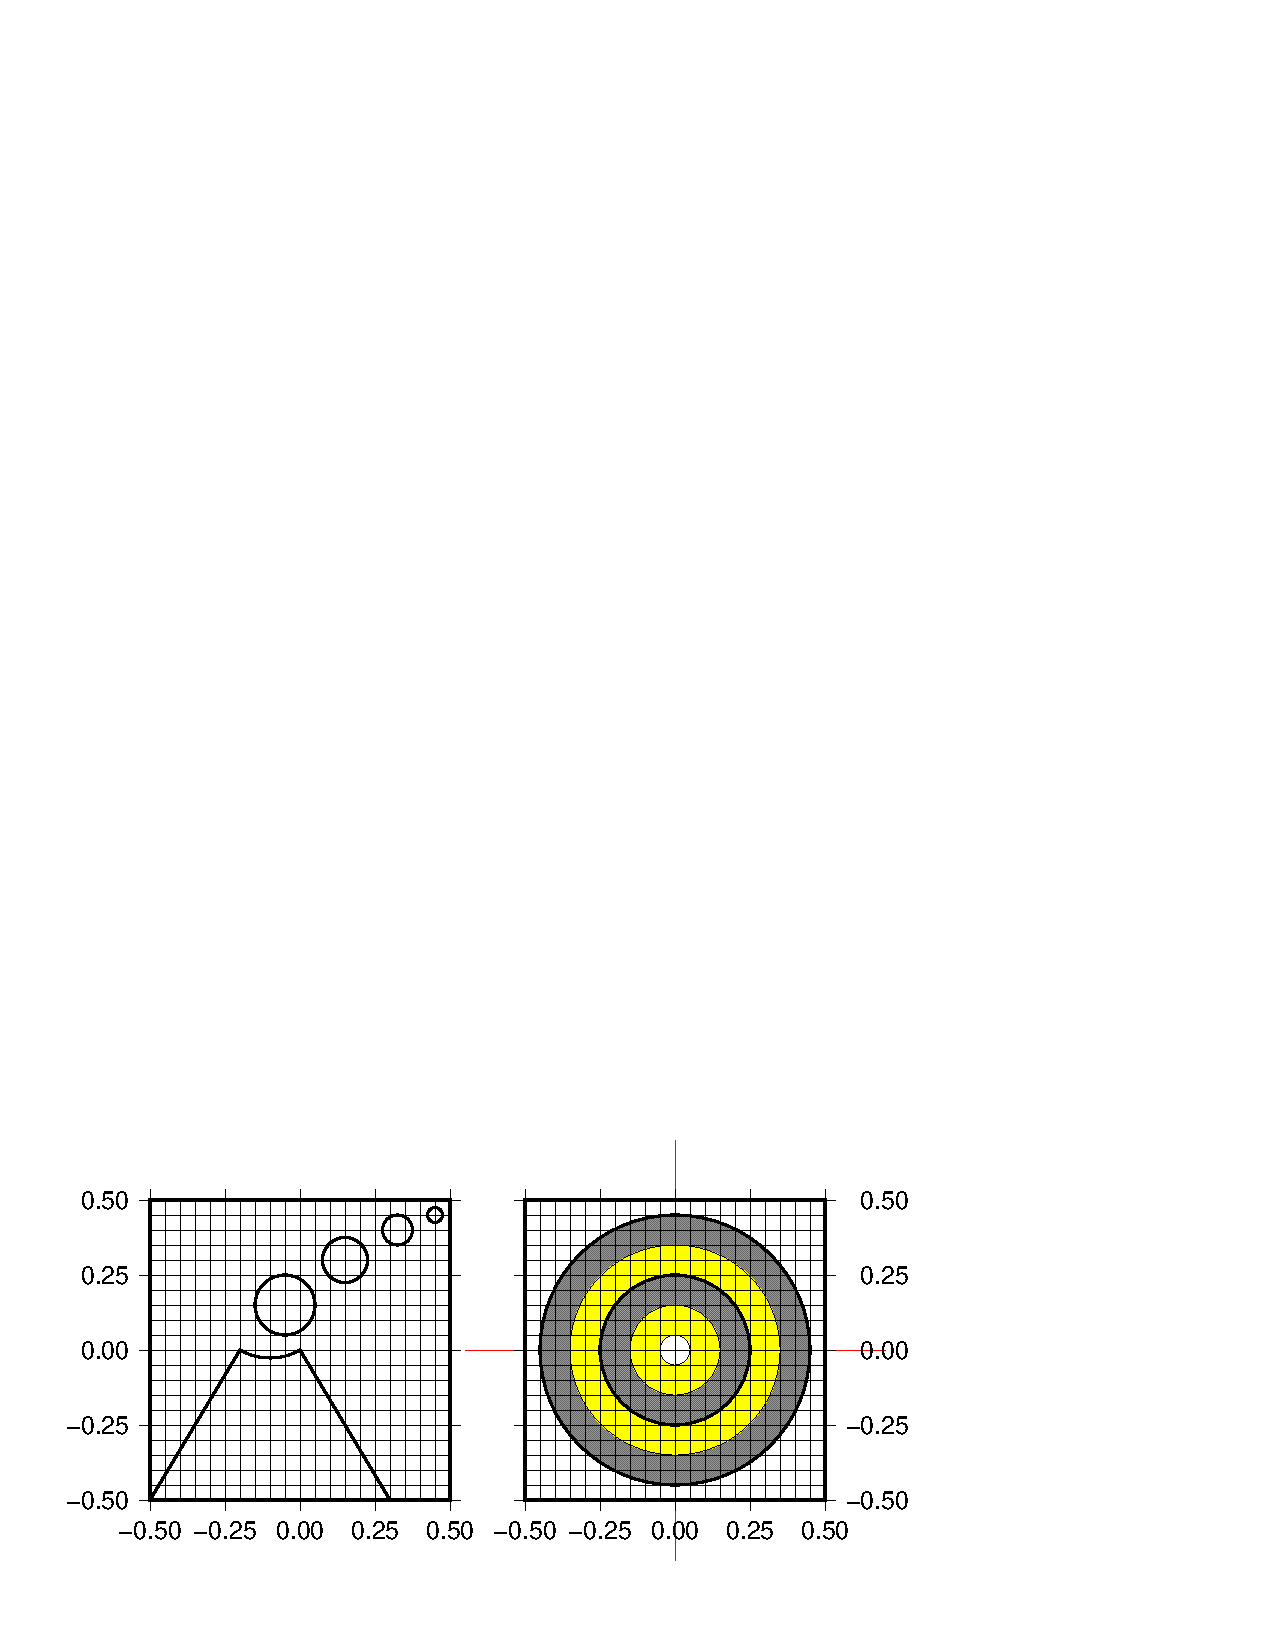
\includegraphics{scripts/GMT_volcano}
\end{figure}

\item After designing the symbol we will encode it using a
simple set of rules.  In our case we describe our volcano and bulls eye
using these three freeform polygon generators:

\begin{tabbing} 
$x_0$ $y_0$ $r$ {\bf C} [ \Opt{G}{\it fill} ] [ \Opt{W}{\it pen} ] \=Draw \kill
$x_0$ $y_0$ {\bf M} [ \Opt{G}{\it fill} ] [ \Opt{W}{\it pen} ] \> Start new element at $x_0$, $y_0$ \\ 
$x_1$ $y_1$ {\bf D} \> Draw straight line from current point to $x_1$, $y_1$ around ($x_0$, $y_0$) \\ 
$x_0$ $y_0$ $r$ $\alpha_1$ $\alpha_2$ {\bf A} \> Draw
arc segment of radius $r$ from angle $\alpha_1$ to $\alpha_2$
\end{tabbing} 

We also add a few stand-alone circles (for other symbols, see \GMTprog{psxy} man page):

\begin{tabbing} 
$x_0$ $y_0$ $r$ {\bf C} [ \Opt{G}{\it fill} ] [ \Opt{W}{\it pen} ] \=Draw \kill
$x_0$ $y_0$ $r$ {\bf c} [ \Opt{G}{\it fill} ] [ \Opt{W}{\it pen} ] \> Draw
single circle of radius $r$ around $x_0$, $y_0$ \\
\end{tabbing} 

The optional \Opt{G} and \Opt{W} can be used to hardwire
the color fill and pen for segments (use {\bf --} to disallow
fill or line for any specific feature).  By default the segments
are painted based on the values of the command line settings.

Manually applying these rules to our volcano symbol results in a
definition file \filename{volcano.def}:

\script{volcano} 

Without much further discussion we also make a definition file \filename{bullseye.def} for a multi-colored bulls eye symbol.
Note that the symbol can be created beyond the -0.5 to +0.5 range, as shown by the red lines. There is no limit in
\GMT\ to the size of the symbols. The center, however, will always be at (0,0). This is the point to which the
coordinates in \GMTprog{psxy} refers.

\script{bullseye} 

The values refer to positions and dimensions illustrated in the Figure above.

\item Given proper definition files we may now use them with \GMTprog{psxy} or \GMTprog{psxyz}.
\end{enumerate}

We are now ready to give it a try.  Based on the hotspot
locations in the file \filename{hotspots.d} (with a 3rd column
giving the desired symbol sizes in inches) we lay down a
world map and overlay red volcano symbols using our custom-built
volcano symbol and \GMTprog{psxy}. We do something similar with the bulls eye symbols.
Without the \Opt{G} option, however, they get the colors defined in \filename{bullseye.def}.

Here is our final map script that produces Figure~\ref{fig:GMT_example_20}:

\script{example_20}
\GMTexample{20}{Using custom symbols in \gmt.}

Given these guidelines you can easily make your own symbols.
Symbols with more than one color can be obtained by making
several symbol components.  E.g., to have yellow smoke coming
out of red volcanoes we would make two symbols: one with just
the cone and caldera and the other with the bubbles.  These
would be plotted consecutively using the desired colors.
Alternatively, like in \filename{bullseye.def}, we may
specify colors directly for the various segments.  Note that
the custom symbols (Appendix~\ref{app:N}), unlike the built-in symbols in \GMT, can
be used with the built-in patterns (Appendix~\ref{app:E}).  Other
approaches are also possible, of course.
\index{Example!custom map symbols|)}

\section{Time-series of RedHat stock price}
\index{Example!RedHat stock price|(}

As discussed in Section~\ref{sec:timeaxis}, the annotation of time-series
is generally more complicated due to the extra degrees of freedom afforded
by the dual annotation system.  In this example we will display the trend
of the stock price of RedHat (RHAT) from their initial public offering until
late 2006.  The data file is a comma-separated table and the records
look like this:
\begin{verbatim}
Date,Open,High,Low,Close,Volume,Adj.Close*
12-Mar-04,17.74,18.49,17.67,18.02,4827500,18.02
11-Mar-04,17.60,18.90,17.37,18.09,7700400,18.09
\end{verbatim}
Hence, we have a single header record and various prices in USD for each
day of business.  We will plot the trend of the opening price as a red line superimposed on
a yellow envelope representing the low-to-high fluctuation during each day.  We
also indicate when and at what cost Paul Wessel bought a few shares, and zoom in
on the developments since 2004; in the inset we label the time-axis in Finnish in honor
of Linus Thorvalds.  Because the time coordinates are Y2K-challenged and the
order is backwards (big units of years come \emph{after} smaller units like
days) we must change the default input/output formats used by \GMT. Finally,
we want to prefix prices with the \$ symbol to indicate the currency.  Here is
how it all comes out:

\script{example_21} 

which produces the plot in Figure~\ref{fig:GMT_example_21}, suggesting Wessel
has missed a few trains if he had hoped to cash in on the Internet bubble...

\GMTexample{21}{Time-series of RedHat stock price since IPO.}

\index{Example!RedHat stock price|)}

\section{World-wide seismicity the last 7 days}
\index{Example!world-wide seismicity|(}

The next example uses the command-line tool \progname{wget} to obtain a data file
from a specified URL\footnote{You can also use the utility \progname{curl}}.
In the example script this line is commented out so the
example will run even if you do not have \progname{wget} (we use the supplied
\filename{neic\_quakes.d} which normally would be created by \progname{wget}); remove the comment to
get the actual current seismicity plot using the live data.  The main purpose of
this script is not to show how to plot a map background and a few circles, but
rather demonstrate how a map legend may be composed using the new tool \GMTprog{pslegend}.
Some scripting is used to pull out information from the data file that is later
used in the legend.  The legend will normally have the email address of the script
owner; here that command is commented out and the user is hardwired to ``GMT guru''.
The USGS logo, taken from their web page and converted to a Sun raster file, is used
to spice up the legend.

\script{example_22} 
\GMTexample{22}{World-wide seismicity the last 7 days.}

The script produces the plot in Figure~\ref{fig:GMT_example_22}, giving the URL
where these and similar data can be obtained.

\index{Example!world-wide seismicity|)}

\section{All great-circle paths lead to Rome}
\label{sec:example_23}
\index{Example!paths to Rome|(}

While motorists recently have started to question the old saying ``all roads lead to Rome'',
aircraft pilots have known from the start that only one great-circle path connects the
points of departure and arrival\footnote{Pedants who wish to argue about the ``other''
arc going the long way should consider using it.}.  This provides the inspiration for our next
example which uses \GMTprog{grdmath} to calculate distances from Rome to anywhere on
Earth and \GMTprog{grdcontour} to contour these distances.  We pick five cities that
we connect to Rome with great circle arcs, and label these cities with their names and
distances (in km) from Rome, all laid down on top of a beautiful world map.  Note that
we specify that contour labels only be placed along the straight map-line connecting
Rome to its antipode, and request curved labels that follows the shape of the contours.

\script{example_23} 
\GMTexample{23}{All great-circle paths lead to Rome.}

The script produces the plot in Figure~\ref{fig:GMT_example_23}; note how
interesting the path to Seattle appears in this particular projection (Hammer).
We also note that Rome's antipode lies somewhere near the Chatham plateau (antipodes
will be revisited in Section~\ref{sec:example_25}).

\index{Example!paths to Rome|)}

\section{Data selection based on geospatial criteria}
\index{Example!geospatial criteria|(}

Although we are not seismologists, we have yet another example involving seismicity.
We use seismicity data for the Australia/New Zealand region to demonstrate how we can
extract subsets of data using geospatial criteria.  In particular, we wish to plot
the epicenters given in the file \filename{oz\_quakes.d} as red or green circles.
Green circles should only be used for epicenters that satisfy the following three criteria:
\begin{enumerate}
\item They are located in the ocean and not on land
\item They are within 3000 km of Hobart
\item They are more than 1000 km away from the International Dateline
\end{enumerate}
All remaining earthquakes should be plotted in red.  Rather that doing the selection
process twice we simply plot all quakes as red circles and then replot those that
pass our criteria.  Most of the work here is done by \GMTprog{gmtselect}; the rest
is carried out by the usual \GMTprog{pscoast} and \GMTprog{psxy} workhorses.  Note
for our purposes the Dateline is just a line along the 180\DS\ meridian.

\script{example_24} 
\GMTexample{24}{Data selection based on geospatial criteria.}

The script produces the plot in Figure~\ref{fig:GMT_example_24}.  Note that the
horizontal distance from the dateline seems to increase as we go south; however that
is just the projected distance (Mercator distortion) and not the actual distance
which remains constant at 1000 km.

\index{Example!geospatial criteria|)}

\section{Global distribution of antipodes}
\label{sec:example_25}
\index{Example!distribution of antipodes|(}

As promised in Section~\ref{sec:example_23}, we will study antipodes.  The antipode of a point at
$(\phi, \lambda)$ is the point at $(-\phi, \lambda + 180)$.  We seek an answer
to the question that has plagued so many for so long: Given the distribution of
land and ocean, how often is the antipode of a point on land also on land? And
what about marine antipodes?  We use \GMTprog{grdlandmask} and \GMTprog{grdmath}
to map these distributions and calculate the area of the Earth (in percent)
that goes with each of the three possibilities.  To make sense of our \GMTprog{grdmath}
equations below, note that we first calculate a grid that is +1 when a point and its
antipode is on land, -1 if both are in the ocean, and 0 elsewhere.  We then
seek to calculate the area distribution of dry antipodes by only pulling out the nodes
that equal +1.  As each point represent an area approximated by $\Delta \phi \times \Delta \lambda$
where the $\Delta \lambda$ term's actual dimension depends on $\cos (\phi)$, we need
to allow for that shrinkage, normalize our sum to that of the whole area of the Earth,
and finally convert that ratio to percent.  Since the $\Delta \lambda$, $\Delta \phi$ terms
appear twice in these expressions they cancel out, leaving the somewhat
intractable expressions below where the sum of $\cos (\phi)$ for all $\phi$ is known to equal $2N_y / \pi$:

\script{example_25}

In the end we obtain a funny-looking map depicting the antipodal distribution as
well as displaying in legend form the requested percentages (Figure~\ref{fig:GMT_example_25}).
Note that the script is set to evaluate a global 30 minute grid for expediency ($D = 30$), hence
several smaller land masses that do have terrestrial antipodes do not show up.  If you want
a more accurate map you can set the parameter $D$ to a smaller increment (try 5 and wait a
few minutes).

The call to \GMTprog{grdimage} includes the \Opt{-Sn} to suspend interpolation and only
return the value of the nearest neighbor. This option is particularly practical for plotting
categorical data, like these, that should not be interpolated.

\GMTexample[width=\textwidth]{25}{Global distribution of antipodes.}

\index{Example!distribution of antipodes|)}

\section{General vertical perspective projection}
\index{Example!vertical perspective projection|(}

Next, we present a recent extension to the \Opt{JG} projection option which allows the user
to specify a particular altitude (this was always at infinity before), as well as several
further parameters to limit the view from the chosen vantage point.  In this example we show
a view of the eastern continental US from a height of 160 km.  Below we add a view with a specific tilt of
55\DS\ and azimuth 210\DS; here we have chosen a boresight twist of 45\DS.  We view the land from
New York towards Washington, D.C.

\script{example_26}

At this point the full projection has not been properly optimized and the map annotations will need
additional work.  Also, note that the projection is only implemented in \GMTprog{pscoast} and \GMTprog{grdimage}.
We hope to refine this further and extend the availability of the full projection to all of the
\GMT\ mapping programs.

\GMTexample{26}{General vertical perspective projection.}
 
\index{Example!vertical perspective projection|)}

\section{Plotting Sandwell/Smith Mercator img grids}
\index{Example!Mercator img grids|(}

Next, we show how to plot a data grid that is distributed in projected form.  The gravity and
predicted bathymetry grids produced by David Sandwell and Walter H. F. Smith are not geographical
grids but instead given on a spherical Mercator grid.  The \GMT\ supplement imgsrc has tools to
extract subsets of these large grids.  If you need to make a non-Mercator map then you must extract
a geographic grid using \GMTprog{img2grd} and then plot it using your desired map projection.
However, if you want to make a Mercator map then you can save time and preserve data quality by
avoiding to re-project the data set twice since it is already in a Mercator projection.  This example
shows how this is accomplished.  We use the \Opt{M} option in \GMTprog{img2grd}\footnote{You could
also use \GMTprog{img2mercgrd} directly -- your only option under DOS} to pull out the
grid in Mercator units (i.e., do \emph{not} invert the Mercator projection) and then simply plot the
grid using a linear projection with a suitable scale (here 0.25 inches per degrees of longitude).
To overlay basemaps and features that has geographic longitude/latitude coordinates we must remember
two key issues:
\begin{enumerate}
	\item This is a \emph{spherical} Mercator grid so we must use {\bf --ELLIPSOID}=Sphere with all
	commands that involve projections (or use \GMTprog{gmtset} to change the setting).
	\item Select Mercator projection and use the same scale that was used with the linear projection.
\end{enumerate}

\script{example_27}

This map of the Tasman Sea shows the marine gravity anomalies with land painted black.  A color scale bar
was then added to complete the illustration.

\GMTexample{27}{Plotting Sandwell/Smith Mercator img grids.}
 
\index{Example!Mercator img grids|)}


\section{Mixing UTM and geographic data sets}
\index{Example!Mixing UTM and geographic data|(}

Next, we present a similar case: We wish to plot a data set given in UTM coordinates and want it
to be properly registered with overlying geographic data, such as coastlines or data points.  The
mistake many \GMT\ rookies make is to specify the UTM projection with their UTM
data.  However, that data have already been projected and is now in linear meters.  The only
sensible way to plot such data is with a linear projection, yielding a UTM map.  In this step one can
choose to annotate or tick the map in UTM meters as well.  To plot geographic (lon/lat) data on
the same map there are a few things you must consider:
\begin{enumerate}
	\item You need to know the lower left and upper right UTM coordinates of your map. Given
	the UTM zone you can use \GMTprog{mapproject} to recover the lon/lat of those two points.
	Conversely, if you instead know the lon/lat corners then you need to convert those
	to UTM coordinates.  You now have the ability to specify two domains with the \Opt{R} setting:
	The linear UTM meter domain when plotting UTM data and the geographic domain (remember to use the
	rectangular variant of \Opt{R} that ends with the modifier {\bf r}) when plotting lon/lat data.
	\item Make sure you use the same scale (and not width) with both the linear and UTM projection.
\end{enumerate}

\script{example_28}

Our script illustrates how we would plot a UTM grid of elevations near Kilauea volcano on the Big Island
of Hawaii.  Given we are in UTM zone 5Q, the script determines the geographic coordinates of the
lower left and upper right corner of the UTM grid, then uses that region when overlaying the coastline
and light blue ocean.  We place a scale bar and label Kilauea crater to complete the figure.

\GMTexample{28}{Mixing UTM and geographic data sets requires knowledge of the map region domain in both
UTM and lon/lat coordinates and consistent use of the same map scale.}
 
\index{Example!Mixing UTM and geographic data|)}

\section{Gridding spherical surface data using splines}
\index{Example!Gridding spherical surface data using splines|(}

Next, we demonstrate how gridding on a spherical surface can be accomplished using Green's functions
of surface splines, with or without tension.  Global gridding does not work particularly well in
Cartesian coordinates hence the chosen approach.  We use \GMTprog{greenspline} to produce a crude
topography grid for Mars based on radii estimates from the Mariner 9 and Viking Orbiter spacecrafts.
This data comes from \emph{Smith and Zuber} [Science, 1996] and is used here as a small (\emph{N} = 370) data set we
can use to demonstrate spherical surface gridding.  Since \GMTprog{greenspline} must solve a \emph{N} by \emph{N}
matrix system your system memory may impose limits on how large data sets you can handle; also note that
the spherical surface spline in tension is particularly slow to compute.

\script{example_29}

Our script must first estimate the ellipsoidal shape of Mars from the parameters given by \emph{Smith and Zuber}
so that we can remove this reference surface from the gridded radii.  We run the gridding twice: First with
no tension using \emph{Parker}'s [1990] method and then with tension using the \emph{Wessel and Becker} [2008] method.
The grids are then imaged with \GMTprog{grdimage} and \GMTprog{grdcontour} and a color scale is placed between
them.

\GMTexample{29}{Gridding of spherical surface data using Green's function splines.}
 
\index{Example!Gridding spherical surface data using splines|)}

\section{Trigonometric functions plotted in graph mode}
\index{Example!Trigonometric functions plotted in graph mode|(}

Finally, we end with a simple mathematical illustration of sine and cosine, highlighting the
{it graph} mode for linear projections and the new curved vectors for angles.

\script{example_30}

The script simply draws a graph basemap, computes sine and cosine and plots them as lines, then
indicates on a circle that these quantities are simply the projections of an unit vector on the
x- and y-axis, at the given angle.

\GMTexample{30}{Trigonometric functions plotted in graph mode.}
 
\index{Example!Trigonometric functions plotted in graph mode|)}
